\documentclass[border={0.1cm 0.1cm 0.1cm 0.1cm}]{standalone}  %E,S,W,N

\usepackage{amssymb}
\usepackage{amsmath}
\usepackage{tikz}
\usetikzlibrary{calc}	%for centerarc

\def\centerarc[#1](#2)(#3:#4:#5) {\draw[#1] ($(#2)+({#5*cos(#3)},{#5*sin(#3)})$) arc (#3:#4:#5);}

\begin{document}
	
	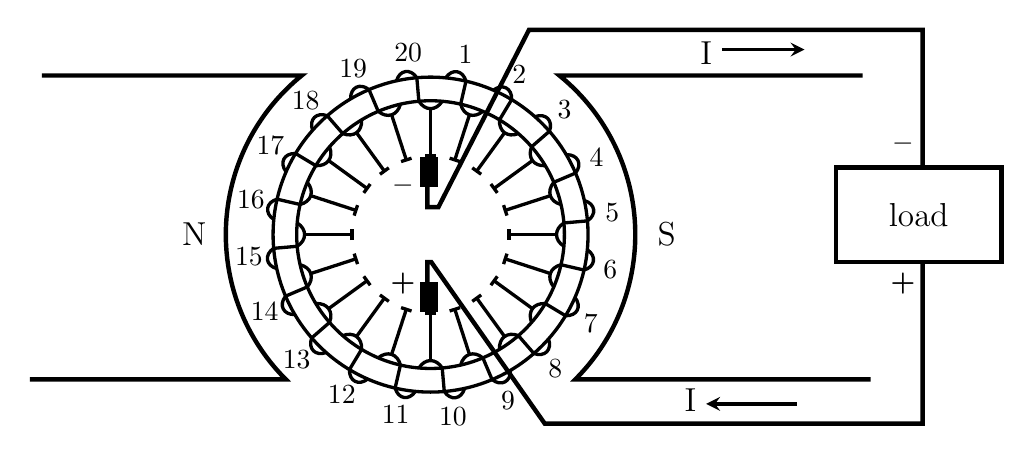
\begin{tikzpicture}[very thick]
	%CIRCLES
	\draw (0,0) circle (1.7cm);
	\draw (0,0) circle (2cm);
	\centerarc[->,>=stealth](0,0)(115:68:2.6)
	
	\foreach \i in {1,...,20}{
		\node at ({2.325*cos(97-18*\i)},{2.325*sin(97-18*\i)}) {\i};
		\draw ({1*cos(94-18*\i)},{1*sin(94-18*\i)})--({1*cos(86-18*\i)},{1*sin(86-18*\i)});
		\draw ({1*cos(90-18*\i)},{1*sin(90-18*\i)})--({1.6*cos(90-18*\i)},{1.6*sin(90-18*\i)});
		\draw ({1.7*cos(95-18*\i)},{1.7*sin(95-18*\i)}) .. controls ({1.57*cos(92.5-18*\i)},{1.57*sin(92.5-18*\i)}) and ({1.57*cos(87.5-18*\i)},{1.57*sin(87.5-18*\i)}) .. ({1.7*cos(85-18*\i)},{1.7*sin(85-18*\i)});
		\draw ({1.7*cos(95-18*\i)},{1.7*sin(95-18*\i)})--({2*cos(95-18*\i)},{2*sin(95-18*\i)});
		\draw ({2*cos(95-18*\i)},{2*sin(95-18*\i)}) .. controls ({2.13*cos(96.875-18*\i)},{2.13*sin(96.875-18*\i)}) and ({2.13*cos(100.625-18*\i)},{2.13*sin(100.625-18*\i)}) .. ({2*cos(102.5-18*\i)},{2*sin(102.5-18*\i)});
	}
	
	%WIRE THING
	\draw[ultra thick] (-0.04,-0.7)--(-0.04,-0.35)--(0.01,-0.35)--(1.45,-2.4)--(6.25,-2.4)--(6.25,2.6)--(1.25,2.6)--(0.1,0.35)--(-0.04,0.35)--(-0.04,0.7);
	\fill (-0.14,0.6) rectangle (0.1,0.98);
	\fill (-0.14,-0.6) rectangle (0.1,-0.98);
	
	%SIDES
	\draw[ultra thick] ({3.75+2.6*cos(-45)},{2.6*sin(-45)})--++(-3.75,0) arc (-45:51:2.6)--++(3.85,0);
	\draw[ultra thick,xscale=-1] ({3.25+2.6*cos(-45)},{2.6*sin(-45)})--++(-3.25,0) arc (-45:51:2.6)--++(3.3,0);
	
	%LABELS
	\node at (-0.35, 0.62) {\bfseries $-$};
	\node at (-0.35,-0.62) {\bfseries +};
	\node at (-3,0) {\large N};
	\node at (3,0) {\large S};
	\node at (3.5,2.3) {\large I};
	\draw[->,>=stealth] (3.7,2.35)--(4.75,2.35);
	\node at (3.3,-2.1) {\large I};
	\draw[->,>=stealth] (4.65,-2.15)--(3.5,-2.15);
	\node at (6,1.15) {\bfseries $-$};
	\draw[ultra thick,fill=white] (5.15,-0.35) rectangle (7.25,0.85);
	\node at (6.2,0.25) {\large load};
	\node at (6,-0.62) {\bfseries +};
	\end{tikzpicture}
	
\end{document}